\begin{frame}{Akash feedback on 17.08.2018}
\begin{itemize}
\item Since \alert{Encrypt Flip-Flop} paper already exists, just pushing the XOR gate inside the flip-flop will be very weak contribution, \alert{still we can include because it is novel}
\item Focus on Dummy Lock-up Latch Insertion and encryption of all lock-up latches (both original and dummy)
\item Design an encrypted lock-up latch, which is negative-level-sensitive when control is \alert{0}, and positive-level-sensitive when control is \alert{1}
\item Lock-up latches across (clock) domains are easily understood, so not easy to encrypt. However, lock-up latches within a (clock) domain are not easily understood without detailed clock simulation, hence possible to introduce dummy ones and encrypt to fool the attacker. So, we focus on encryption of lock-up latches within a (clock) domain. 
\end{itemize}
\end{frame}

\begin{frame}{Proposed Experiments (Positive-Edge-Triggered Design)}
	\begin{itemize}
		\item SAT attack has to be launched through EDT BYPASS mode
%		\item Assume Positive-Edge-Triggered design
		\item Since all scan-chains are daisy-chained, surely there will be lot of lock-up latches (because scan chains that are widely spread across SoC are connected, so heavy skew). For these cases, use encrypted lock-up latchwith control=0
		\item Add extra dummy lock-up latches at places where they are not required, however for these cases, use encrypted lock-up latch with control=1
		\item The attacker will not know which are real and which are dummy. 
			\begin{itemize}
				\item \alert{Reason}: Not all far-apart scan-cell-pairs need a lockup latch. So, not easy for attacker to figure out which are real and which are dummy, and hence the correct key. 
			\end{itemize}
	\end{itemize}
\end{frame}

\begin{frame}{Proposed Experiments}
\begin{itemize}
	\item Need placement information of all scan-cells
	\item Currently, have access def files of all ITC benchmarks (without scan cells)
	\item \alert{Assumption}: Consider coordinates of the gate driven by the scan cell, as the coordinate of the scan cell
	\item \texttt{b19} has 6.6K scan cells, so 
	\begin{itemize}
		\item if taking maximum 500 scan cells in one-chain (industry practice), there will be 13 scan-chains
		\item if taking maximum 300 scan cells in one-chain, there will be 22 scan-chains
		\item if taking maximum 100 scan cells in one-chain, there will be 66 scan-chains

	\end{itemize}
\end{itemize}
\end{frame}

\begin{frame}{Proposed Experiments}
\begin{itemize}
	\item Fix maximum chain length to desired value, and use coordinates to cluster them into multiple chains using machine learning. 
	\item Connect the chains successively, through end scan cells. 
	\item Do clock tree simulation (Use Timing book)
	\begin{itemize}
		\item add lockup latches within each chain where necessary
		\item add lock-up latches where necessary between chain-chain connections
	\end{itemize}
	\item Add dummy lock-up latches finally. 
\end{itemize}
\end{frame}

\begin{frame}{Proposed Additional Experimental flow for lock-up latches}
	\begin{figure}[!htbp]
		\begin{center}
		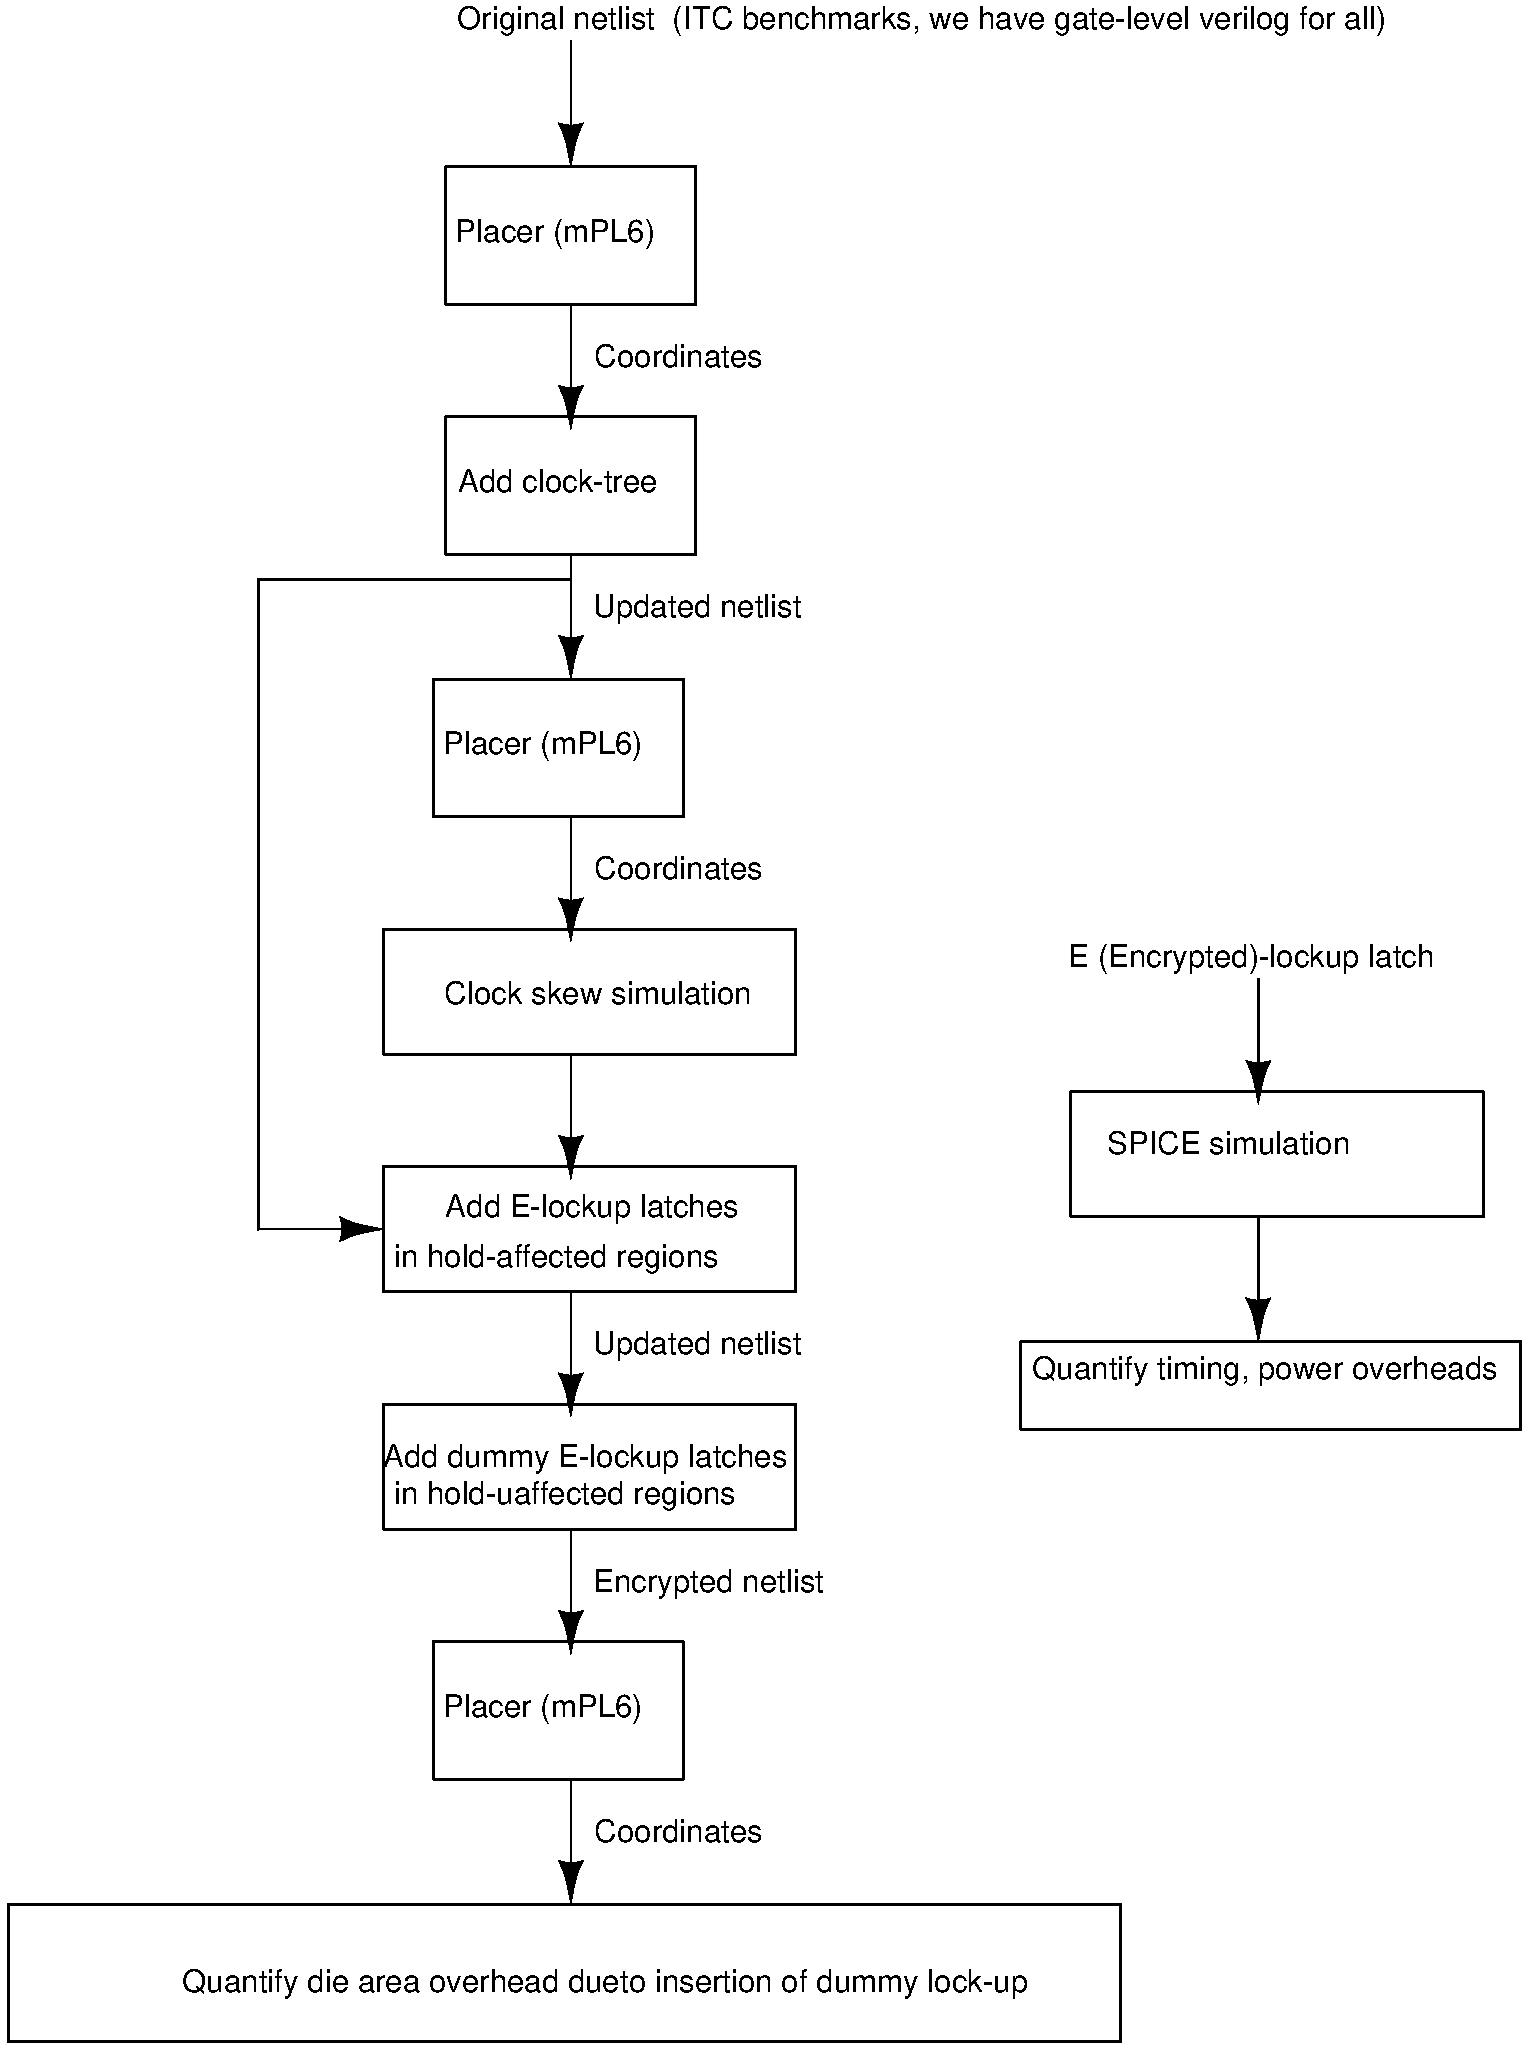
\includegraphics[scale=0.16]{fig/experiments-flow.pdf}
		\end{center}
	\end{figure}
\end{frame}
